\documentclass[binding=0.6cm, LaM]{sapthesis}
\usepackage{microtype}
\usepackage[english]{babel}
\usepackage[utf8]{inputenx}
\usepackage{hyperref}
\usepackage{wasysym}
\usepackage{siunitx}
\hypersetup{pdftitle={My thesis},pdfauthor={Giada Caneva Santoro}}
\usepackage{amsmath, amssymb}
\title{Building a template bank}
\author{Giada Caneva Santoro}
\IDnumber{1490713}
\course{Facoltà di Scienze Matematiche Fisiche e Naturali}
\courseorganizer{Corso di Laurea Magistrale in Fisica}
\AcademicYear{2018/2019}
\copyyear{2012}
\advisor{Prof. Francesco Pannarale Greco}
\authoremail{giada.greenday92@gmail.com}

\begin{document}

\frontmatter
\maketitle
\dedication{Dedicated to \\ me, whom I have been to hell and back.}

\begin{abstract}
In the present work we describe the methodology to build a template bank for one of the gravitational wave searches that will be carried out in the LIGO-Virgo interferometers observation campaign. We will also quantify the effectiveness of detection using the most current waveform models and characterise the fraction of signals not detected in the common approximation in which the template bank is built neglecting the emission in ways superior to the fundamental one.
\end{abstract}

\tableofcontents

\mainmatter 
\chapter{Introduction}
\section{Gravitational waves in linearized gravity}
\subsection{Weak-field metric}
In 1915, Albert Einstein presented his general theory of relativity  which describes how mass distorts spacetime and in turn how spacetime dictates how masses flow through it. The classical Newtonian notion of gravity ,which stated that gravity arises from an action at a distance, was replaced with a geometric interpretation of the Universe, the spacetime continuum: it can be regarded as a fabric and it can be curved by the mass of an object. Masses moving on this curved spacetime fabric will then be perceived as gravity. 
In general relativity, space-time is regarded as a four-dimensional manifold with a Lorentzian metric, and gravity is a manifestation of the manifold’s curvature. The spacetime curvature is associated with the stress-energy tensor of matter fields through the Einstein’s field equations:

\begin{equation}
G_{\mu\nu} \equiv R_{\mu\nu}  - {1 \over 2}g_{\mu\nu}R = {8\pi G_{N} \over {c^4}}T_{\mu\nu} 
\end{equation}

Where $G_{\mu\nu} $ is the Einstein tensor, $T_{\mu\nu} $ is the stress-energy tensor of matter-fields and $ G_{N}$ is Newton’s gravitational constant. 

General relativity predicts that gravity is mediated by a new type of radiation: gravitational radiation. In 1916 Einstein found the weak-field solutions to general relativity had wave-like solutions, gravitational waves. 
Gravitational waves that compose gravitational radiation are ripples in the fabric of spacetime, which periodically lengthen and shorten space, and speed up and slow down time. 



 To study the properties of gravitational waves, it is instructive to first study them in situations where the gravitational fields are weak. In the so-called weak-field approximation, one can view the metric as the Minkowski metric with a small perturbation: it is required to expand the Einstein equations around the flat-space metric, considering as a perturbation on the space-time of special relativity. Letting $ x_\mu = (t, x, y, z)$ denote the time and space coordinates, we can write the proper distance between events $x_{\mu}$ and
$x_{\mu} + dx_{\mu}$ as
\[
ds^2 = g_{\mu\nu}dx^{\mu}dx^{\nu} \approx (\eta_{\mu\nu} + h_{\mu\nu})dx_{\mu}dx_{\nu}. \hspace*{2cm}\|h_{\mu\nu}\|\ll 1
\]
Here $\eta_{\mu\nu} = diag(-1,1,1,1)$ is the usual Minkowski metric and
 $h_{\mu\nu}$ represents the linearised gravitational field.
The metric perturbation is referred to as  $h_{\mu\nu}$: it encapsulates gravitational waves, but contains additional, non-radiative degrees of freedom as well; $\|h_{\mu\nu}\|$ means “the magnitude of a typical non-zero component of $h_{\mu\nu}$”. The condition $\|h_{\mu\nu}\|\ll 1$ requires both the gravitational field to be weak, and in addition constrains the coordinate system to be approximately Cartesian.  In linearized gravity, the smallness of the perturbation means that only terms which are linear in $h_{\mu\nu}$ are considered; higher order terms are discarded. As a consequence, indices are raised and lowered using the flat metric. The metric perturbation $h_{\mu\nu}$ transforms as a tensor under Lorentz transformations, but not under general coordinate transformations: since the numerical values of the components of a tensor depend on the reference frame, there exists a reference frame where the linearisation of the gravitational field holds on a sufficiently large region of the spacetime. 
The Einstein field equations are covariant under general coordinate transformations
\begin{equation}
x^{\mu} \rightarrow x^{\mu ‘}(x)
\end{equation}


So that the metric transforms as 
\begin{equation}
g_{\mu\nu} \rightarrow g_{\mu' \nu'} = x^{\rho},_{\mu'}x^{\sigma},_{\nu'}g_{\rho \sigma}
\end{equation}


This means that one is free to choose a convenient coordinate system without altering the physical predictions of the field equations. Choosing a reference frame breaks the invariance of general relativity under coordiante trasformations but it also erases spurious degrees of freedom.
However,after choosing a frame where the field is linearised, a residual gauge symmetry remains. Under infinitesimal coordinate transformations
 $x_{\mu} \rightarrow x_{\mu} + \xi_{\mu}$:

Using the transformation law of the metric, to lowest order $h_{\mu\nu}$ transforms as
\[
h_{\mu\nu} \rightarrow h_{\mu\nu} - \partial_{\mu}\xi_{\nu} - \partial_{\nu}\xi_{\mu}
\]
\subsection{Linearising the Einstein field equations}
All the fundamental quantities in the field equations need to be computed in order to linearise the theory. Rather than working with the metric perturbation, changing notation and using the trace-reversed perturbation makes the computation more compact and cleaner. Defining 
\begin{equation}
{\bar h}_{\mu\nu} = h_{\mu\nu} - {1 \over {2}}\eta_{\mu\nu}h  
\end{equation}
and the trace 
\begin{equation}
h = \eta^{\mu\nu}h_{\mu\nu}
\end{equation}
expressing the trace-reversed field:
\begin{equation}
h_{\mu\nu} = {\bar h}_{\mu\nu} + {1 \over {2}}\eta_{\mu\nu}{\bar h}
\end{equation} 
The Rienmann tensor constructed in linearised theory is given by
\begin{align}

R^{\mu}_{\nu\rho\sigma} = \partial_{\rho} \Gamma^{\mu}_{\nu\sigma} - \partial_{\sigma}\Gamma^{\mu}_{\nu\rho}  \\
&={ 1 \over 2} (\partial_{\rho}\partial_{\nu}h^{\mu}_{\nu\rho} + \partial_{\sigma}\partial^{\mu}h^{\nu\rho} - \partial_{\rho}\partial^{\mu}h^{\nu\sigma} - \partial_{\sigma}\partial_{\nu}h^{\mu}_{\rho})

\end{align}
From this, the Ricci tensor takes the form
\begin{equation}
R_{\mu\nu} = R^{\rho}_{\mu\rho\nu} = {1 \over 2}(\partial_{\rho}\partial{\nu}h^{\rho}_{\mu} + \partial^{\rho}\partial_{\mu}h_{\nu\rho} - \square h_{\mu\nu} - \partial_{\mu}\partial_{\nu}h)
\end{equation}
The curvature scalar is obtained contracting once more:
\begin{equation}
R = R^{\mu}_{\mu} = (\partial_{\rho}\partial^{\mu}h^{\rho}_{\mu} - \square h)
\end{equation}

Combining all together the Einstein tensor can be expressed as
\begin{equation}
G_{\mu\nu} = {1 \over 2}(\partial_{\rho}\partial{\nu}h^{\rho}_{\mu} + \partial^{\rho}\partial_{\mu}h_{\nu\rho} - \sqaure h_{\mu\nu} - \partial_{\mu}\partial_{\nu}h - \eta_{\mu\nu}\partial_{\rho}\partial^{\sigma}h^{\rho}_{\sigma} + \eta_{\mu\nu}\square h)
\end{equation}
Substituting the metric perturbation $h_{\mu\nu}$  with the $trace-reversed$ perturbation ${\bar h}_{\mu\nu}$ and expandig, the linerised Einstein equations assume the  compact form:
\begin{equation}
\square {\bar h}_{\mu\nu} + \eta_{\mu\nu}{\partial}^{\rho}{\partial}^{\sigma}{\bar h}_{\rho\sigma} - {\partial}^{\rho}{\partial}^{\nu}{\bar h}_{\mu\rho} - {\partial}^{\rho}{\partial}^{\mu}{\bar h}_{\nu\rho} = - {{16\pi G_{N}} \over {c^4}}T_{\mu\nu}.
\end{equation}


The linearised equations of motion are gauge-invariant, and the gauge freedom can
 be used to simplify the form of the field equations.
 In the Lorentz family of gauges, choosing the harmonic gauge 
 $ \partial_{\mu}h_{\mu\nu} = 0 $ 
 , reduces the Einstein equations to a simple wave equation that relates the trace-reversed field
 to the stress energy tensor:
\begin{equation}
\square {\bar h}_{\mu\nu} =({\partial^2 \over {\partial t^2} } - {\partial^2 \over {\partial x^2}}  - {\partial^2 \over {\partial y^2}}  -  {\partial^2 \over {\partial z^2}}) {\bar h}_{\mu\nu} = -{{16\pi G_{N}} \over {c^4}}T_{\mu\nu}. 
\end{equation}
By imposing the harmonic gauge one has chosen the coordinates in such a way that for a single plane wave (or a superposition of plane waves with their wave vectors pointing in the same direction), the GW polarisations are perpendicular to the direction of propagation.

The harmonic gauge gives four conditions, that reduce the 10 indipendent component of the symmetric 4x4 matrix $h_{\mu\nu}$ to six indipendent component, so it does not fix the gauge completely, leaving 4 additional components free to be gauge-fixed.  
If the metric perturbation is not in the harmonic gauge, by making an infinitesimal coordinate transformation 
\begin{equation}
{\bar h}_{\mu\nu} \rightarrow {\bar h}_{\mu’\nu’}  = {\bar h}_{\mu\nu}  - \xi_{\mu,\nu} -\xi_{\nu,\mu} + \eta_{\mu\nu}\xi^{\rho}_{,\rho}
\end{equation}
and applying the harmonic gauge condition

\begin{equation}
{\bar h}_{\mu’\nu’,} ^{\nu’} = {\bar h}_{\mu\nu,} ^{\nu} - \xi_{\mu,\nu}^{\nu}
\end{equation}

Therefore any metric perturbation can be put into an harmonic gauge by making an infinitesimal coordinate transformation that satisfies 
\begin{equation}
{\bar h}_{\mu\nu,} ^{\nu} = \xi_{\mu,\nu}^{\nu}
\end{equation}

This is a wave equation that always admits a solution, thus one can always achieve the harmonic gauge. 

Outside the source where $T_{\mu\nu} = 0$ 

\begin{equation}
\square {\bar h}_{\mu\nu} = 0
\end{equation}

In vacuum spacetimes which are asymptotically flat ($h_{\mu\nu} \rightarrow 0 as r \rightarrow 0$), along with choosing the harmonic gauge, the metric perturbation can be greatly simplified using the residual gauge freedom within the harmonic gauge class. The transverse-traceless gauge,  $TT$-gauge, can be obtained by choosing the components of the metric tensor $h_{\mu\nu}$, so that only the ones on the plane orthogonal to the direction of propagation (transverse) are different from zero, this results in $h_{\mu\nu}$ being traceless:

\begin{equation}
h^{0\mu} = 0 \hspace*{0.5cm}  h^{i}_i = 0  \hspace*{0.5cm}   {\partial}^jh_{ij} = 0
\end{equation}

By imposing the harmonic gauge, the 10 degrees of freedom of the symmetric matrix $h_{\mu\nu}$ have reduced to six degrees of freedom, and the residual gauge freedom, associated to the four functio $\xi^{\mu}$, has further reduced these to just two degrees of freedom, which corrispond to the two possible polarization states of the gravitational wave. 
Equation (1.16) has plane wave solutions, $h_{\mu\nu}^{TT}(x)=e_{ij}(k)e^{ikx}$ with $k^{\mu}=(w/c,k)$ and $w/c=|k|$. The tensor $e_{ij}(k)$ is called the polarization tensor. In vacuum spacetimes, a plane gravitational wave with a given wave-vector $k$ is characterized by two functions $h_+$ and $h_{\times}$, while the remaining components can be set to zero by choosing the transverse-traceless gauge. Choosing $n$ along the z axis:

\begin{equation} 
h_{\mu\nu}^{TT} = 
\begin{bmatrix}
0 & 0 & 0 & 0 \\
0 & h_{+} & h_{\times} & 0 \\
0 & h_{\times} & -h_{+} & 0 \\
0 & 0 & 0 & 0 
\end{bmatrix}cos[w(t-z/c)]
\end{equation}
\chapter{Interaction of Gravitational waves with test masses}
To understand how gravitational waves interact with the detectors, mirrors in the case of the interferometric detectors, it's necessary to use the geodesic equation and the geodesic deviation equation, which are also important tools for understanding the physical meaning of a given gauge choice. In fact the physics must be invariant under coordinate trasformations but GWs and the detector description's depend on the chosen reference frame. 
\section{Geodesic equation and geodesic deviation}
The usual notion of “gravitational force” disappears in general relativity, replaced instead by the idea that freely falling bodies follow geodesics in spacetime. 
Geodesics are the curved-space equivalents of straight lines, which can be found by parallel transporting the tangent vector of a curve.
Given a spacetime metric $g_{\mu\nu}$ and a set of spacetime coordinates $x^{\mu}$, geodesic trajectories are given by the equation: 
\begin{equation}
{{d^2x^{\mu}}\over{d\tau^2}} + \Gamma_{\nu\rho}^{\mu}(x){{dx^{\nu}}\over{d\tau}}{{dx^{\rho}}\over{d\tau}} = 0 \hspace*{2cm} m \neq 0
\end{equation}
\begin{equation}
{{d^2x^{\mu}}\over{d\lambda^2}} + \Gamma_{\nu\rho}^{\mu}(x){{dx^{\nu}}\over{d\lambda}}{{dx^{\rho}}\over{d\lambda}} = 0 \hspace*{2cm} m = 0
\end{equation}
which is the classical equation of motion of a test mass in the curved background described by the metric $g_{\mu\nu}$, in the absence of external non gravitational force and where $m$ is the mass of the object, $\tau$ represents the proper time given by $d\tau^2 = −ds^2$, and $\lambda$ is some affine parameter on the geodesic. 
In a flat spacetime, two straight lines taht are initially parallel to each other will remain parallel. In a curved spacetime, geodesics do not satisfy this property. Instead, two nearby geodesics, separeted by $\zeta^{\mu}$, follow the geodesic deviation equation
\begin{equation}
{{D^2\zeta^{\mu}}\over{D\tau^2}} = -R^{\mu}_{\nu\rho\sigma}\zeta^{\rho}{{dx^{\nu}}\over{d\tau}}{{dx^{\sigma}}\over{d\tau}}
\end{equation}
where $D/D\tau$ is defined as 
\begin{equation}
{{DV^{\mu}}\over{D\tau}} \equiv {{dV^{\mu}}\over{dtau}} + \Gamma^{\mu}_{\nu\rho}V^{\nu}{{dx^{\rho}}\over{d\tau}}
\end{equation}
and denotes the covariant derivative along a curve that is parameterised by $\tau$. The geodesic deviation equation describes the change in separation $\zeta^{\mu}$ between two nearby geodesic. As the Rienmann tensor describes the tidal forces caused by the gravitational field, the geodesic deviation equation shows that these tidal forces can be considered as deviations of nearby geodesics.

\subsection{Transverse-traceless gauge}
Consider a test mass initially at rest at $\tau = 0$. The geodesic equation then becomes
\begin{equation}
{{dx^i}\over{d\tau^2}} = -[\Gamma^i_{\nu\rho}{{dx^{\nu}}\over{d\tau}}{{dx^{\rho}}\over{d\tau}}]_{\tau=0} \\ 
= - [ \Gamma^i_{00}({{dx^0}\over{d\tau}})^2]_{\tau=0}
\end{equation}
by assumption
\begin{equation}
{{dx^i}\over{d\tau}} = 0 \hspace*{2cm} at \hspace*{0.5cm}\tau = 0
\end{equation}
since the mass is initially at rest. Expanding to first order in $h_{\mu\nu}$, the Christoffel symbol $\Gamma^i_{00}$ vanishes in the TT gauge
\begin{equation}
 \Gamma^i_{00} = {1 \over {2}}(2\partial_{0}h_{0i} - \partial_i h_{00})
\end{equation}
because both $h_{00}$ and $h_{0i}$ are set to zero by the gauge condition. Therefore, if at time $\tau = 0$ $dx^i/d\tau$ is zero, remains zero at all times, because its derivatives also vanishes. 
This shows that if two test masses are initially separated by a coordinate separation of $x^i$ in the TT frame, and are at rest with respect to each other, they will remain at this separation. Overall, it seems that a GW has no influence on the geodesic or on the deviation of geodesics. 
In other words, in the TT gauge the coordinate location of a slowly moving, freely falling body is unaffected by the GW because the coordinates move with the waves.
The TT gauge illustrates that, in general relativity, the physical effects are not expressed by what happens to the coordinates since the theory is invariant under coordinate transformations: the position of test masses doesn't change because the freedom of gauge allowed to define the coordinates in such a way that they don't change. Physical effects can instead be found monitoring proper distances, or proper times. 

In fact the GWs cause the
proper separation between two freely falling particles to oscillate, even if the coordinate
separation is constant. Consider two spatial freely falling particles, located at $z = 0$, and separated on the x axis by a coordinate distance $L_c$. Consider a GW in TT gauge that propagates down the z axis, $h^{TT}_{\mu\nu}(t,z)$. The proper distance L between the two particles in the presence of the GW is given by
\begin{align}
L & = \int^{L_c}_{0}{dx\sqrt{g_{xx}}} = \int^{L_c}_{0}dx\sqrt{1 + h^{TT}_{xx}(t,z=0)} \\
 & \simeq \int^{L_c}_{0}{dx[1 + {1 \over 2}h^{TT}_{xx}(t,z=0)]} \\
&= L_c[1 + {1 \over 2}h^{TT}_{xx}(t,z=0)]
\end{align}
Therefore, the proper distance expands and shrinks periodically,with a fractional length change $\delta L/L$ given by
\begin{equation}
{{\delta L}\over{L}} \simeq {1 \over 2} h_{xx}^{TT}(t,z=0)
\end{equation}
Even though this result is calculaterd in the TT gauge, it is indeed gauge indipendent.$h_{xx}^{TT}$acts as a strain, a fractional length change.
 Because the time that light travels between the two test masses is related to the proper distance,  which directly relates to the accumulated phase measured by laser interferometric GW observatories, GWs leave an imprint on the time it takes for a photon to make a round trip. Consequently, interferometers can potentially measure these imprints by measuring the length difference between their arms. The “extra” phase $\delta \phi$ (if $L \ll \lambda$ so that the metric perturbation does not change value very much during a light travel time) accumulated by a photon that travels down and back the arm of a laser interferometer in the presence of a GW is $\delta \phi = 4\pi \delta L \lambda$, where $\lambda$ is the photon’s wavelength and $\delta L$ is the distance the end mirror moves relative to the beam splitter. 

\subsection{Local proper reference frame}

A convenient coordinate system for analyzing the geodesic deviation equation is the local proper reference frame of the observer who travels along the first geodesic. y, consider a detector capable of measuring changes in the proper distance, e.g. an interferometer, with a characteristic size that is much smaller than the characteristic wavelength of the GW. In this case, one can approximate the entire detector to be in a near local Lorentz frame  (freely falling frame), even in the presence of GWs. This coordinate system is defined by the requirements
\begin{equation}
z^i(\tau) = 0, \hspace*{2cm} g_{ab}(t, 0) = \eta_{ab}, \hspace*{2cm} \Gamma^a_{bc}(t,0) = 0,
\end{equation}
which imply that the metric has the form

\begin{equation}
ds^2 \approx -dt^2 + \delta_{ij}dx^i dx^j + O({{x^ix^j}\over{L^2_B}})
\end{equation}
where $L^2_B$ denotes the typical variation scale of the metric.
Consider now the proper distance between the two geodesics, $\zeta^i$, to understand how the GWs influence these two test masses the geodesic deviation equation is calculated as 
\begin{equation}
{{d^2\zeta^{\mu}}\over{d\tau^2}} + 2\Gamma^{\mu}_{\nu\rho}{{dx^{\nu}}\over{d\tau}}{{dx^\rho}\over{d\tau}} + \zeta^{\sigma}\Gamma^{\mu}_{\nu\rho,\sigma}{{dx^{\nu}}\over{d\tau}}{{dx^{\rho}}\over{d\tau}} = 0
\end{equation}
Assuming the two test masses are moving non-relativistically, $dx^i/d\tau$ can be neglected compared to $dx^0/d\tau$. Furthermore, the term proportional to $\Gamma^{\mu}_\nu\rho{}$ is negligible compared to other terms in a near LLF. Hence,
\begin{equation}
{{d^2\zeta^{\mu}}\over{d\tau^2}} + \zeta^{\sigma}\Gamma^{i}_{00, \sigma}({{dx^0}\over{d\tau}})^2 = 0
\end{equation}
Further simplifying $\zeta^{\sigma}\Gamma^{i}_{00, \sigma} \approx \zeta^{j}\Gamma^{i}_{00, j}$
\begin{equation}
{{d^2\zeta^{\mu}}\over{d\tau^2}} + \zeta^{j}\Gamma^{i}_{00,j}({{dx^0}\over{d\tau}})^2 = 0
\end{equation}
But in the LLF, $R^i_{0j0} = \Gamma^i_{00,j} - \Gamma^i_{0j,0} = \Gamma^i_{00,j}$ and therefore
\begin{equation}
{{d^2\zeta^{\mu}}\over{d\tau^2}} + R^i_{0j0} \zeta^j({{dx^0}\over{d\tau}})^2 = 0
\end{equation}
Because $dx^0/d\tau \approx 1$, one can approximate $\tau \approx t$:
\begin{equation}
{\ddot \zeta}^j = - R^i_{0j0}\zeta^j
\end{equation}
The key quantity entering into the equation, the Rienmann tensor, is gauge invariant in linearized theory, it can be evaluated in any convenient coordinate system. The expression for the Rienmann tensor in terms of the TT gauge metric perturbation $h_{ij}^TT$
\begin{equation}
R^i_{0j0} = R_{i0j0} = - {1 \over 2}{\ddot h}_{ij}^{TT}
\end{equation}
Substituting into the previous equation, the geodesic deviation equation in the proper detector frame takes the form
\begin{equation}
{\ddot \zeta}^i = {1 \over 2}{\ddot h}_{ij}^{TT}\zeta^j
\end{equation}
which can be interpreted as if the influence of a GW in a near LLF resembles a Newtonian force.
In general directions, the proper distance is given by
\begin{equation}
s = \sqrt{L^2 + h_{ij}(t)L_{i}L_{j}}
\end{equation}
where $L_i$ denotes the spatial separation between two test masses and $L$ the associated coordinate distance.
In the given metric for the proper reference frame, the proper distance is just $|L| = \sqrt{L_iL_j}$ up to fractional errors; since the only detectors taken in consideration are those with $L \ll \lambda$, these errors are smaller than the fractional distance changes caused by the GW. Therefore $|L|$ is simply identified as the proper separation. The ideal equation for analyzing an interferometric GW detector is
\begin{equation}
{\ddot L}^i = {1 \over 2}{\ddot h}_{ij}^{TT}L^j
\end{equation}
 
\subsection{Ring of test masses}
The effects of gravitational waves cannot be seen in isolated bodies. This is a result of
the fact that a single test mass, in a frame freely falling with it, will remain at rest. At
least two test masses are required to measure the effects of gravitational waves. This is also
the case when one wants to measure any curvature of spacetime. 
Consider a ring of test masses in the $(x, y)$ plane of a proper detector frame, initially at rest, centred at $z = 0$, and a GW travelling in the $z$-direction. This situation restricts the attentionto the $(x,y)$ plane alone, because $h_{ij}^{TT}$ is transverse to the propagation direction, so the GW will only have influence in the plane of the test masses: the only non zero compontents of the metric perturbation are
\begin{equation}
h_{xx}^{TT} = - h_{yy}^{TT} = h_{+} \hspace*{3cm} h_{xy}^{TT} = h_{yx}^{TT} = h_{\times}
\end{equation}
where $h_{+}(t-z)$ and $h_{\times}(t-z)$ are the two polarization components, which are indipendent and can be considered separately.
For the plus polarization at $z=0$ and initial conditions $h_{ij}^{TT} = 0$ at $t=0$:
\begin{equation}
h_{ab}^{TT} = 
\begin{bmatrix}
1  & 0 \\
0 &  -1 \\
\end{bmatrix} 
h_{+}cos \omega t
\end{equation}

If the displacement between geodesics is $\zeta_a (t) = (x_0 + \delta x(t), y_0 + \delta y(t))$, then of $\zeta_a (t)$ is 

\begin{equation}
\delta {\ddot x} = - {{h_{+}} \over 2} (x_0 + \delta x) \omega ^2 sin \omega t
\end{equation}
\begin{equation}
\delta {\ddot y} =  {{h_{+}} \over 2} (y_0 + \delta y) \omega ^2 sin \omega t
\end{equation}
Assuming that the perturbations are $O(h)$, and thus small compared to the unperturbed locations, $\delta x$ and $\delta y$ can be neglected.
The integrations gives the deviations caused by the plus polarisations:

\begin{equation}
\delta x(t) =  {{h_{+}} \over 2} x_0 sin \omega t
\end{equation}
\begin{equation}
\delta y(t) = - {{h_{+}} \over 2} y_0  sin \omega t
\end{equation}
Similarly, for the cross polarization at $z=0$ and initial conditions $h_{ij}^{TT} = 0$ at $t= 0$, the situation is described by the equations
\begin{equation}
\delta x(t) =  {{h_{\times}} \over 2} y_0 sin \omega t
\end{equation}
\begin{equation}
\delta y(t) =  {{h_{\times}} \over 2} x_0  sin \omega t
\end{equation}
This set of equations describes the changes in the x and y components for a passing gravitational wave. The plus polarization alternately stretches and compresses the ring of test masses in the x and y directions, while the cross polarization exhibits the same behavior rotated by $\ang{45}$ in the x - y plane. 

\begin{figure}
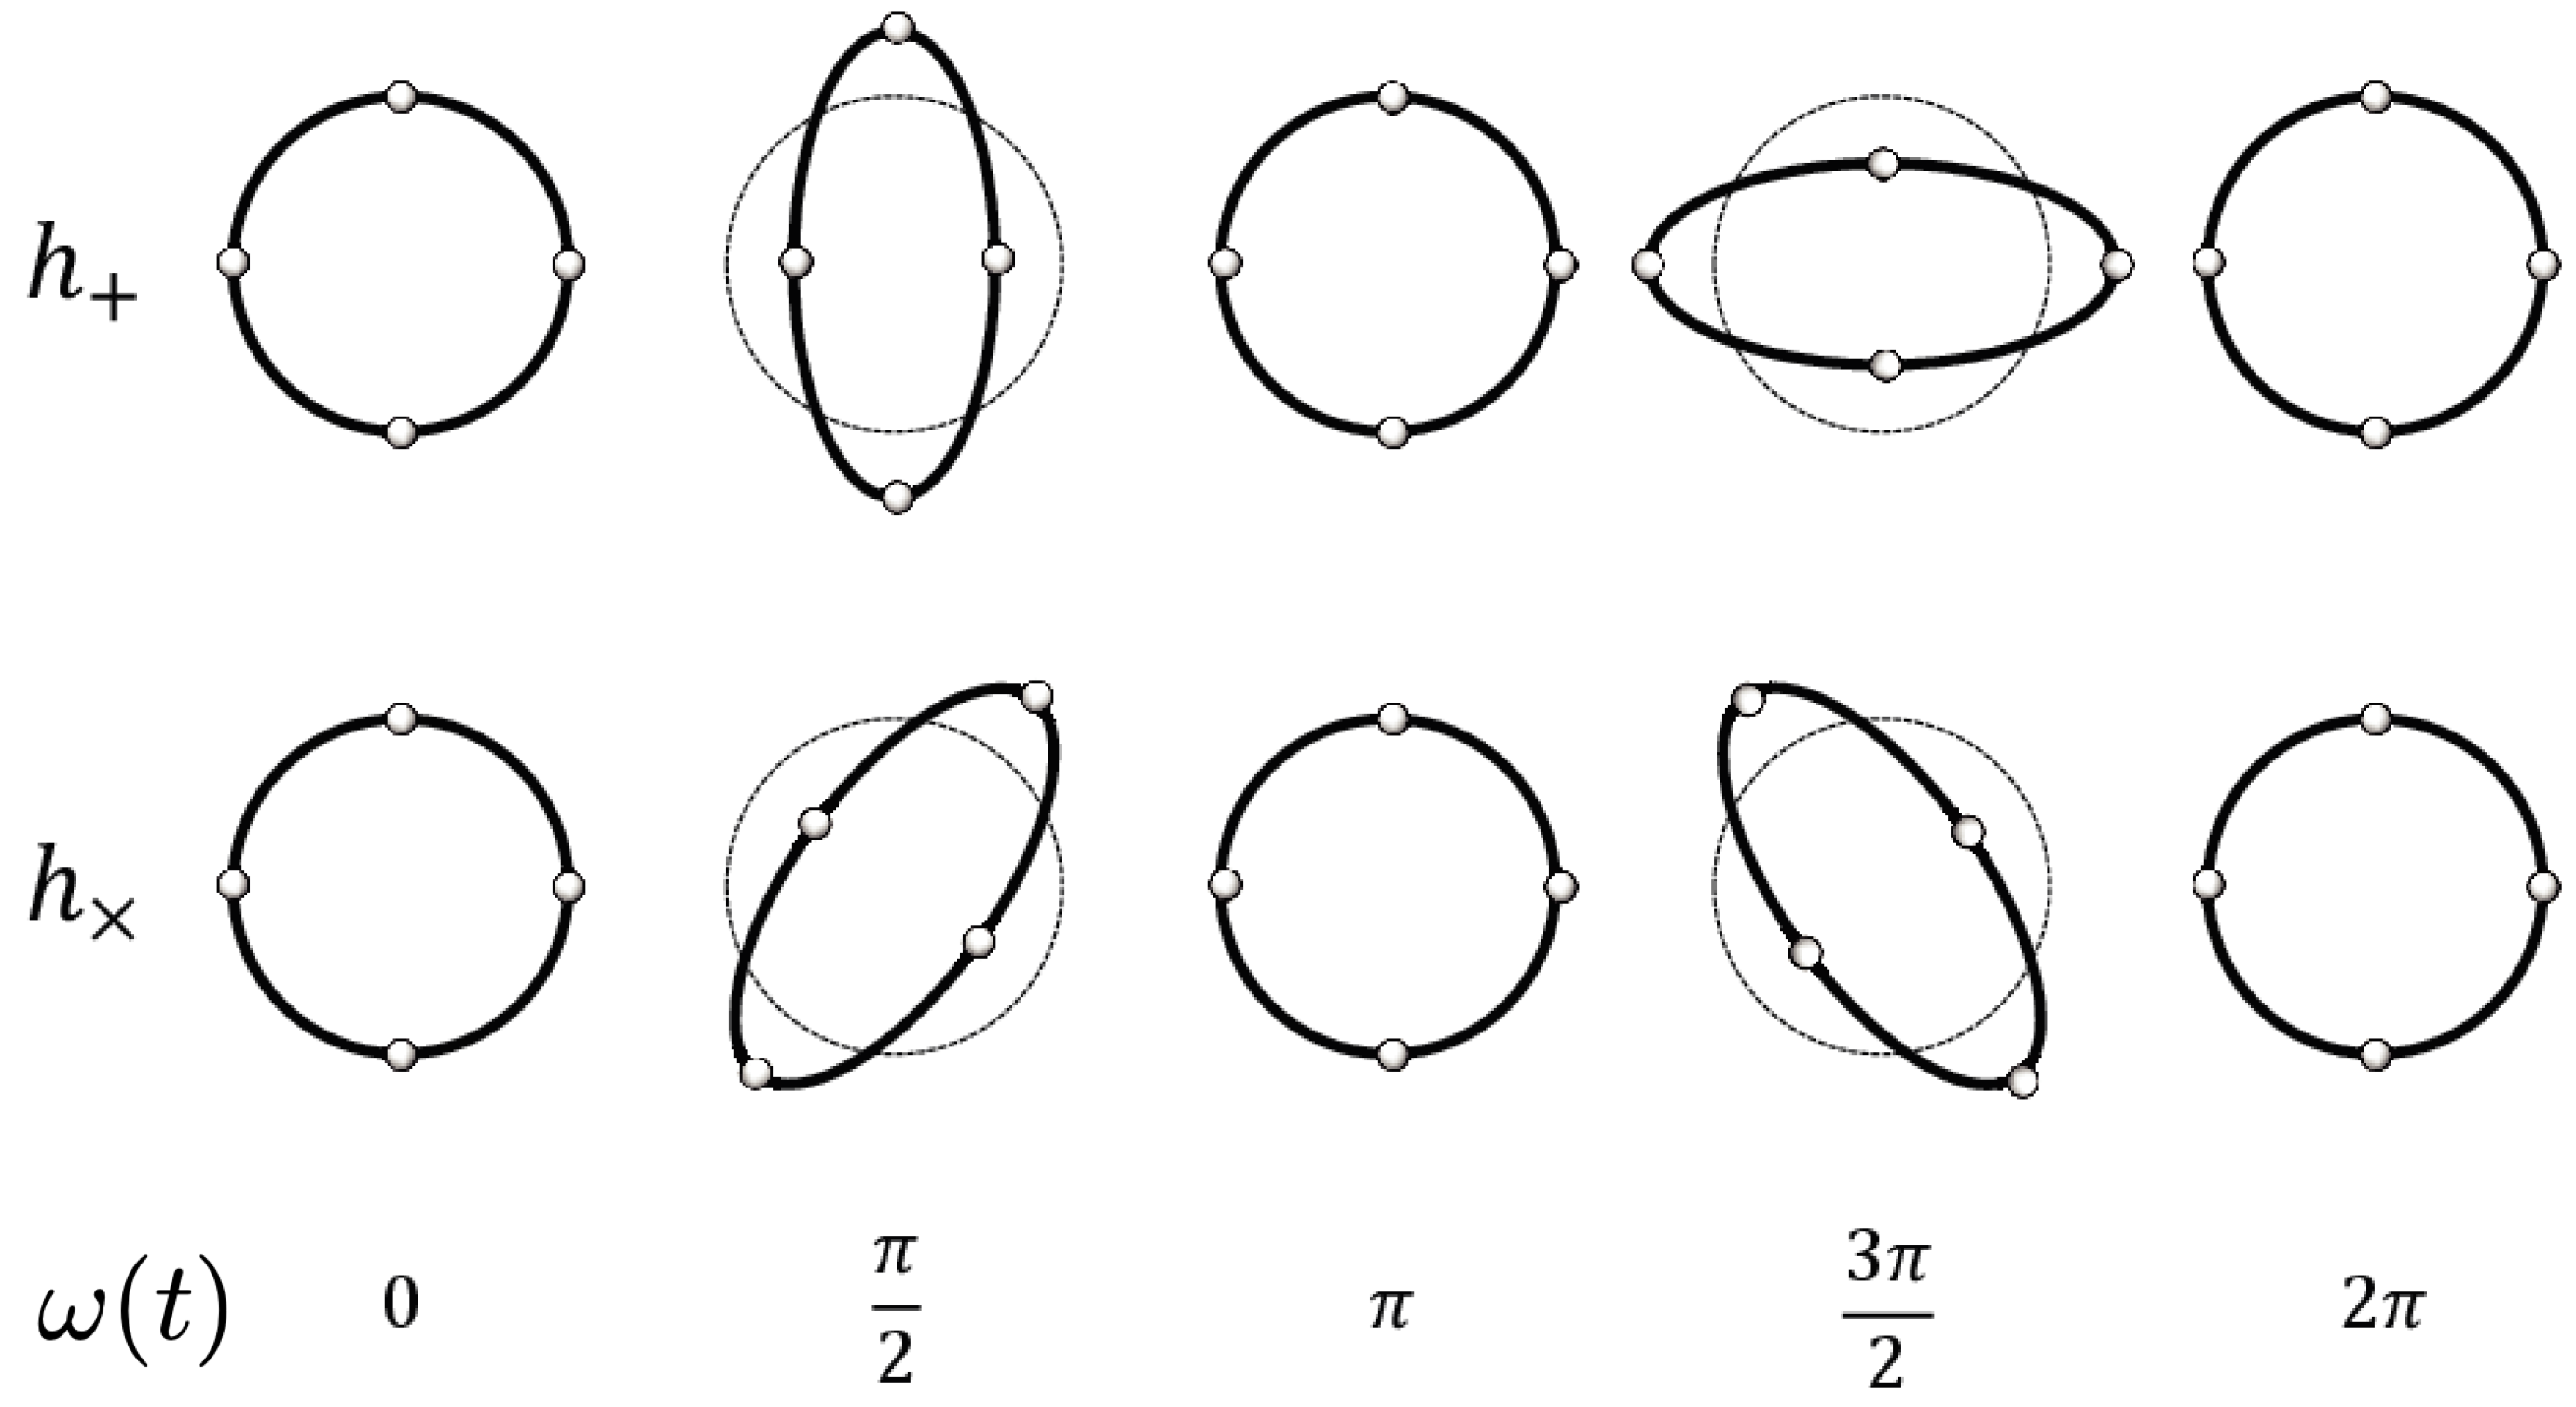
\includegraphics[scale=1]{ring}
\centering
\caption{The effects of plus and cross polarization on a ring of test masses. The plus polar- ization alternately compresses and stretches the x- and y-separations. The cross polarization has the same effect only rotated by  $\ang{45}$.}
\label{fig:ring}
\end{figure}

\subsection{Energy and momentum of gravitational waves}


\subsection{Generation of gravitational waves}

\subsection{Gravitational waves in post-newtonian formalism}

\chapter{Gravitational waves: Detection and sources}
\section{Gravitational waves vs Electromagnetic waves}
The generation and propagation of gravitational and electromagnetic radiation are basically quite similar but, on a more practical level, gravitational and electromagnetic waves are quite different.
First of all, electromagnetic waves interact strongly with matter; GWs do not. 
The weak interaction of GWsmeans that they propagate from emission to Earth-bound observers with essentially zero absorption, making it possible to probe astrophysics that is hidden or dark to electromagnetic observations — e.g., the coalescence and merger of black holes, the collapse of a stellar core, the dynamics of the early Universe. It also means that detecting GWs is very difficult. 

Electromagnetic radiation typically has a wavelength smaller than the size of the emitting system, and so can be used to form an image of the source. This is because electromagnetic radiation is usually generated by moving charges in the environment of some larger source — e.g., an atomic transition in interstellar gas, or emission from hot plasma in a stellar environment. By contrast, the wavelength of gravitational radiation is typically comparable to or larger than the size of the radiating source. GWs are generated by the bulk dynamics of the source itself — e.g., the motion of neutron stars in a binary. As a consequence, GWs cannot be used to form an image: The radiation simply does not resolve the generating system. Instead, GWs are best thought of as analogous to sound — the two polarizations carry a stereophonic description of the source’s dynamics.

Gravitons in a gravitational-wave burst are phase coherent; photons in electromagnetic signals are usually phase-incoherent. This arises from the fact that each graviton is generated from the same bulk motion of matter or of spacetime curvature, while each photon is normally generated by different, independent events involving atoms, ions or electrons. Thus GWs are similar to laser light. We can take advantage of the phase coherence of GWs to enhance their detectability. Matched filtering techniques for detecting GW bursts with well-modeled functional form (like those generated by coalescing compact binaries) extend the distance to which sources can be seen by a factor of roughly the square root of the number of cycles in the waveform, a significant gain.

An extremely important consequence of this coherency is that the direct observable of gravitational radiation is the strain $h$, a quantity that falls off with distance as $1/r$. Most electromagnetic observables are some kind of energy flux, and so fall off with a $1/r^2$ law; measuring coherent GWs is analogous to measuring a coherent, $1/r$ 
electromagnetic radiation field. This comparatively slow fall off with radius means that relatively small improvements in the sensitivity of GW detectors can have a large impact on their science: Doubling the sensitivity of a detector doubles the distance to which sources can be detected, increasing the volume of the Universe to which sources are measurable by a factor of 8. Every factor of two improvement in the sensitivity of a GW observatory should increase the number of observable sources by about an order of magnitude. 
In most cases, electromagnetic astronomy is based on deep imaging of small fields of view: Observers obtain a large amount of information about sources on a small piece of the sky. GW astronomy will be a nearly all-sky affair: GW detectors have nearly $4\pi$ steradian sensitivity to events over the sky. A consequence of this is that their ability to localize a source on the sky is not good by usual astronomical standards; but, it means that any source on the sky will be detectable, not just sources towards which the detector is “pointed”. The contrast between the all-sky sensitivity but poor angular resolution of GW observatories, and the pointed, high angular resolution of telescopes is very similar to the angular resolution contrast of hearing and sight, strengthening the useful analogy of GWs with sound. 
It is useful to categorize GW sources (and the methods for detecting their waves) by the frequency band in which they radiate. Broadly speaking, we may break the GW spectrum into four rather different bands: the ultra low frequency band,$10^{-18}Hz \apprle f \apprle 10^{-13} Hz$; the very low frequency band, $10^{−9} Hz \apprle f \apprle 10^{−7} Hz$; the low frequency band, $10^{−5} Hz \apprle f \apprle 1Hz$; and the high frequency band, $1Hz \apprle f \apprle 10^4 Hz$.

For compact sources, the GW frequency band is typically related to the source’s size $R$ and mass $M$. Here the source size $R$ means the lengthscale over which the source’s dynamics vary; for example, it could be the actual size of a particular body, or the separation of members of a binary. The “natural” GW frequency of such a source is $f_{GW} \sim (1/2\pi)\sqrt{GM/R^3}$. Because $R \apprge 2GM/c^2$ (the Schwarzschild radius of a mass $M$), an upper bound for the frequency of a compact source can be estimated:
\begin{equation}
f_{GW}(M) < {1 \over {4\sqrt{2 \pi}}}{{c^3}\over{GM}} \approx 10^4 Hz ({{M_{\odot}} \over M})
\end{equation}
This is a rather hard upper limit, since many interesting sources are quite a bit larger than $2GM/c^2$, or else evolve through a range of sizes before terminating their emission at $R \approx 2GM/c^2$. Nonetheless, this frequency gives some sense of the types of compact sources that are likely to be important in each band — for example, high frequency compact sources are of stellar mass (several solar masses); low frequency compact sources are thousands to millions of solar masses, or else contain widely separated stellar mass bodies.

\section{High frequency}
The high frequency band, $1Hz \apprle f \apprle 10^4 Hz$, is targeted by the new generation of ground-based laser interferometric detectors such as LIGO. (It also corresponds roughly to the audio band of the human ear: When converted to sound, LIGO sources are audible to humans.) The low frequency end of this band is set by the fact that it is extremely difficult to prevent mechanical coupling of the detector to ground vibrations at low frequencies, and probably impossible to prevent gravitational coupling to ground vibrations, human activity, and atmospheric motions.
The high end of the band is set by the fact that it is unlikely any interesting GW source radiates at frequencies higher than a few kilohertz. Such a source would have to be relatively low mass $(\apprle 1M_{\odot})$ but extremely compact.There are no known theoretical or observational indications that gravitationally collapsed objects in this mass range exist.Several interferometric GW observatories are either operating or being completed in the United States, Europe, Japan, and Australia. Having multiple observatories widely scattered over the globe is extremely important: The multiplicity gives rise to cross-checks that increase detection confidence and also aids in the interpretation of measurements. For example, sky location determination and concomitant measurement of the distance to a source follows from triangulation of time-of-flight differences between separated detectors.
\begin{itemize}
  \item LIGO. The Laser Interferometer Gravitational-wave Observatory[55] consists of three operating interferometers: A single four kilometer interferometer in Livingston, Louisiana, as well as a pair of interferometers (four kilometers and two kilometers) in the LIGO facility at Hanford, Washington. The sites are separated by roughly 3000 kilometers, and are situated to support coincidence analysis of events.
  \item Virgo. Virgo is a three kilometer French-Italian detector under construction near Pisa, Italy which employs a very sophisticated seismic isolation system that promises extremely good low frequency sensitivity.
  \item GEO600. GEO600 is a six hundred meter interferometer constructed by a German-English collaboration near Hanover, Germany . Despite its shorter arms, GEO600 achieves sensitivity comparable to the multi-kilometer instruments using advanced interferometry techniques. This makes it an invaluable testbed for technology to be used in later generations of the larger instruments, as well as enabling it to make astrophysically interesting measurements.
  \item TAMA300. TAMA300 is a three hundred meter interferometer operating near Tokyo. 
   
\end{itemize}

The figure shows the detectors sensitivities and "facility limits", the lowest noise levels that can be achieved even in principle within an interferometer facility. The low level facility limits come from gravity-gradient noise: noise arising from gravitational coupling to fluctuations in the local mass distribution (such as from seismic motions in the earth near the test masses,human activity near the detector , and density fluctuations in the atmosphere At higher frequencies, the facility limit arises from residual gas (mostly hydrogen) in the interferometer vacuum system — stray molecules of gas effectively cause stochastic fluctuations in the index of refraction.
\subsection{Sources}
\subsection{Coalescing compact binaries}
Compact binaries — binary star systems in which each member is a neutron star or black hole — are currently the best understood sources of GWs. Double neutron stars have been studied observationally since the mid 1970s; five such systems tight enough to merge within a few 108 or 109 years have been identified in our Galaxy. Extrapolation from these observed binaries in the Milky Way to the Universe at large indicates that GW detectors should measure at least several and at most several hundred binary neutron star mergers each year (following detector upgrades; the expected rate for initial detectors is of order one event per several years, so that measurement of an event is plausible but of fairly low probability). Population synthesis (modelling evolution of stellar populations) indicates that the measured rate of binaries containing black holes should likewise be interestingly large (perhaps even for initial detectors). The uncertainties of population synthesis calculations are rather large, however, due to poorly understood aspects of stellar evolution and compact binary formation; data from GW detectors is likely to have a large impact on this field. 
\section{GWs Detectors}
As a GW causes the stretching and shrinking of the proper distance between test particles, GWs can be observed by measuring these changes in the proper distance. The influences of GW is measured by interferometers, that are configured to show destructive interference when no distortions are present. When a GW passes such a detector, the configuration will no longer support the destructive interference and a bright spot can be seen. By measuring the intensity of this spot as well as its temporal variation, one will be able to observe the footprints of a GW. 

\begin{figure}
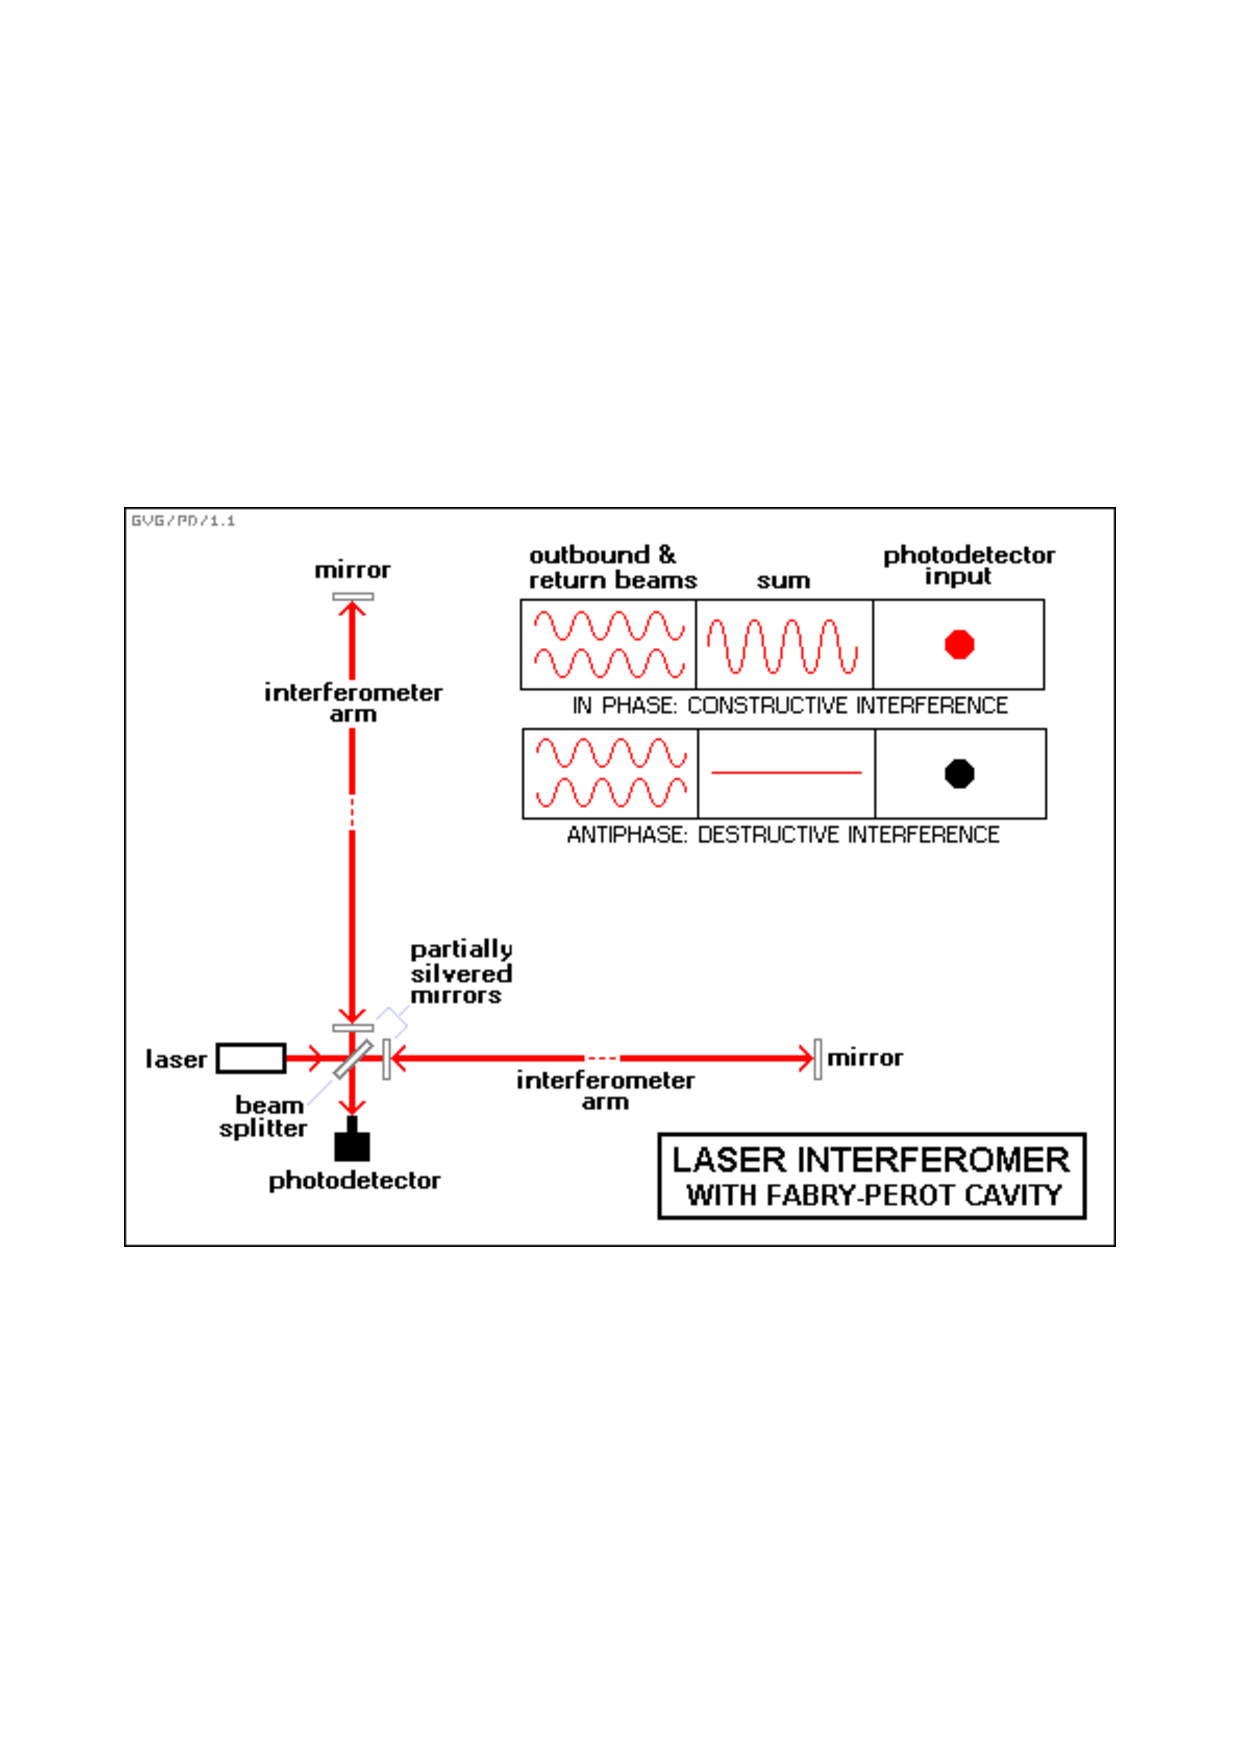
\includegraphics[scale=0.55]{spot}
\centering
\caption{Schematic overview of an interferometric detecto. Without a GW present, the interferometer is kept at a destructive interference configuration. A GW will change the relative distance between the arms and cause the interferometer output to deviate from the destructive interference. The intensity of the light and its temporal evolution encode the footprints of GWs.}
\label{fig:spot}
\end{figure}
The first gravitational wave detectors were resonant-mass cylindrical bar detectors. The first was developed and built by Joseph Weber in the 1960s. Over the course of the next several decades, more bar detectors were built that were at least four orders of magnitude more sensitive than Weber’s original design. These detectors would be set into oscillation at their resonant frequency by passing gravitational waves near that resonant frequency and were sensitive to gravitational waves with relatively high frequency $(\textasciitilde 1 kHz)$ and in a narrow frequency band. In order to detect signals in a broader range of frequencies and out to farther distances, large-scale interferometric detectors have been built. The idea originated with the Russian theorists, M. Gertsenshtein and V. I. Pustovoit in 1962. But the strong push for using interferometers came in the late 1960s with R. Forward, R. Weiss, R. Drever, and others. From the early 2000s, several kilometer-scale ground-based interferometers operated in the frequency band from ∼ 10 Hz to ∼ 1 kHz at a sensitivity that allowed the potential for detection from a variety of sources at large extragalactic distances.
An interferometric detector is based on the simple principles of a Michelson interferometer. In general, an interferometer uses laser light as a displacement measuring device. Two highly reflecting mirrors and a central beam splitter (a 50\% reflecting mirror) act as test masses. The three masses are suspended as pendulums and are allowed to swing freely in the horizontal direction. Thus, they can be considered freely falling masses in that direction. The reflecting mirrors,  labeled as test masses, are placed equidistant from the central beam splitter but in orthogonal directions.
A beam of laser light is incident on the beam splitter and is split into two beams along the x and y arms. The light is then reflected by the end mirrors, recombined at the beam splitter, and detected at the photodiode. When the beams recombine, they will interfere constructively if the lengths of the two arms differ by an integral number of wavelengths and interfere destructively if the lengths differ by an odd number of half wavelengths:

\begin{equation}

\end{equation}
\subsection{Beam pattern functions}
nterferometers are sensitive to the relative difference between two distances, the so-called strain. Suppose we have an interferometer with its arms pointing along the unit vectors $u^i$ and $v^i$. The strain $h(t)$ is given by
\begin{equation}
h(t) = {1 \over 2} (h_{ij}u^iu^j - h_{ij}v^iv^j) = D^{ij}h_{ij}(t)
\end{equation}
where $D^{ij}$ is referred to as the detector tensor and is given by
\begin{equation}
D^{ij} = {1\over 2} (u^iu^j -v^iv^j)
\end{equation}

As the expression for $h(t)$ is linear in $h_{+}$ and $h_{\times}$, one can also write

\begin{equation}
h(t) = F_{+}h_{+} (t) + F_{\times}h_{\times}(t)
\end{equation}
where $F_{+,\times}$ are called the beam pattern functions. Suppose we have a detector with arms that are perpendicular to each other, one pointing in the x-direction and the other in the $y$-direction in a Cartesian coordinate system. This detector frame, denoted by $(x,y,z)$, is generally different from the GW coordinate system, denoted by $(x',y',z')$, where the source is conveniently described. To account for such a difference, we first note that when the plus and cross polarisations are not equal in strength, we can rotate the coordinate system by an angle $\psi$ around the $z′$ axis so that the $x′$ and $y′$ axes coincide with the mayor and minor axis of the associated ellipse. In going from the GW frame to the detector frame, we can rotate the GW frame by an angle $\theta$ around the $x′$ axis and an angle $\phi$ around the $z′$ axis, where the angles $(\theta, \phi)$ denote the direction of propagation of the GW in the detector frame. Applying these three rotations, the beam pattern functions for a detector with perpendicular arms are given by 

\begin{align}
F_{+}^{\ang{90}}& = {1 \over 2} (1 + cos^2 \theta)cos 2\phi cos 2 \psi - cos \theta sin2\phi sin2\psi \\
F_{\times}^{\ang{90}}& = {1 \over 2} (1 + cos^2 \theta)cos 2\phi sin 2 \psi + cos \theta sin2\phi cos2\psi
\end{align}




\subsection{Stellar core collapse}

\subsection{Periodic emitters}

\subsection{Stochastic backgrounds}
\section{Low frequency}
\backmatter
\cleardoublepage

\phantomsection % Give this command only if hyperref is loaded \addcontentsline{toc}{chapter}{\bibname}

\begin{thebibliography}{100}
   \bibitem[nome]{riferimento}
\end{thebibliography}

\end{document} 

